\section{Machbarkeit der Echtzeit-Verhaltensklassifizierung} \label{sec:Ergeb Sim}
Um zu bestätigen, dass eine Echtzeit-Verhaltensklassifizierung umsetzbar ist, muss die Funktionalität des Moduls verifiziert werden. Dazu ist zu untersuchen, ob die Anforderungen erfüllt werden. In diesem Kapitel wird die Anwendungssimulation ausgewertet, um diese Fragen zu beantworten. \par

Überprüft wird, die lückenlose Abtastung des Stallgeschehens und Echtzeitfähigkeit. Dazu findet eine Betrachtung der Laufzeiten statt. Auch die Abtastrate des Moduls wird ermittelt. Der größte Fokus liegt auf der Korrektheit der Schätzung. Es wird untersucht, ob das Modul dazu in der Lage, das Verhalten in der Anwendung korrekt zu bestimmen. \par

Die Simulation wird zweimal durchgeführt, mit jeweils unterschiedlichen Daten. Der erste Durchlauf betrachtet Daten aus einem Kamerabereich, der auch in den Trainingsdaten vorhanden ist. Der zweite Durchlauf betrachtet Daten aus einem zuvor nicht genutzten Kamerabereich. Alle Daten stammen aus dem ersten Mastdurchlauf. Es wird immer ein kompletter Aufzeichnungstag durchlaufen. Das Modul misst während der Verarbeitung die Laufzeiten automatisch. \par

Die Auswertung der erfolgt manuell. Die Videos zu den ausgewählten Daten werden angesehen und dabei werden die Verhaltensweisen notiert. Dadurch entsteht ein Datensatz, welcher als Referenz verwendet wird. Aus dem Ergebnis des Moduls werden die erkannten Kontrollgänge und Kämpfe nochmal gesondert betrachtet, um sicherzugehen, dass die erkannte Verhaltensweise beim Erstellen der Referenz nicht übersehen wurde.\par

\subsection{Auswertung der Laufzeiten}

Die Abbildung \ref{fig:HistGesamt} zeigt ein Histogramm der Gesamtlaufzeiten der Verarbeitung des Moduls.  

\begin{figure}[htb]
    \centering
    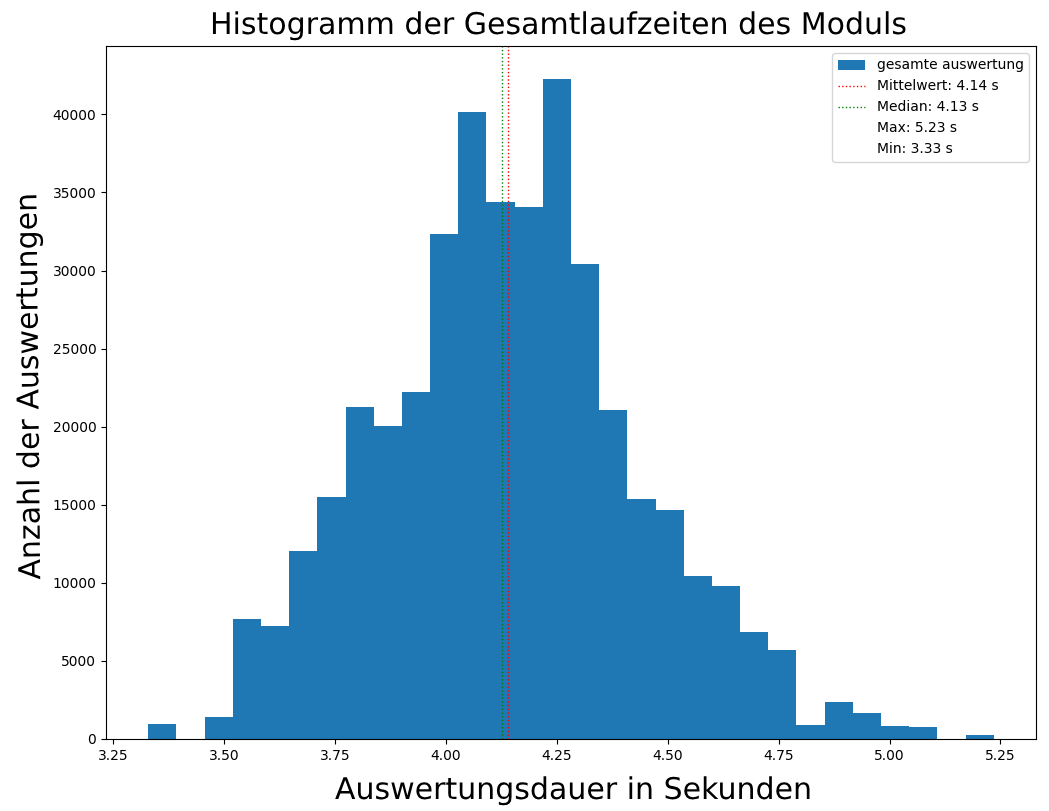
\includegraphics[width=0.9\textwidth]{img/Plots/Simulation/Auswertung Runtimes Histogram gesamte auswertung mit Frames.png}
    \caption{Histogramm der Gesamtlaufzeiten der Verarbeitung.}
    \label{fig:HistGesamt}
\end{figure}

Im Mittel benötigt die Verarbeitung 4,14 Sekunden. Mittelwert und Median liegen dicht bei einander. Die maximale gemessene Verarbeitungsdauer beträgt 5,23 Sekunden. Diese Werte bestätigen, dass eine lückenlose Abtastung des Stallgeschehens realisiert ist. Im Schnitt überlappen die Intervalle fast 36 Sekunden. Das sollte in einer geringen Diskrepanz zwischen dem Auftreten eines Ereignisses und der Erkennung resultieren. Die Verarbeitungszeit bestimmt die Abtastrate des Moduls. Es wird somit alle 4,14 Sekunden abgetastet. \par

Mit diesem Wissen lässt sich die minimale und maximale Dauer bestimmen, die es benötigt, ein Ereignis zu erkennen. Durch die Vorgaben, dass ein Intervall 40 Sekunden umfasst und dass ein Ereignis 30 Sekunden davon einnehmen muss, um erkannt zu werden, lässt sich der Ausdruck in \autoref{eq:deltTErkenn} formulieren. \(D\) ist die Laufzeit des Ereignisses bei einem Abtastzeitpunkt und \(T\) ist die Dauer der Verarbeitung. Läuft das Ereignis exakt 30 Sekunden, umfasst es die Minimalanforderung, um erkannt zu werden. In diesem Fall wird das Ereignis so früh wie für das Modul möglich erkannt. Fällt die Abtastung so, dass das Ereignis gerade so keine 30 Sekunden umfasst, dann resultiert dies in der maximalen Erkennungsdauer. Ausgehend von der maximalen und minimalen Verarbeitungsdauer des Moduls, wird ein Ereignis frühstens nach 33,33 Sekunden erkannt und spätestens nach 40,46 Sekunden.

\begin{equation}
    \label{eq:deltTErkenn}
    \text{Gesamtzeit} = 
    \begin{cases} 
    30 + T & \text{Minimum (} D = 30 \text{ Sekunden)} \\
    D + 2T & \text{Maximum (} D < 30 \text{ Sekunden, nahe an 30)}
    \end{cases}
\end{equation}

 Echtzeitfähigkeit bedeutet, dass ein System innerhalb einer festgelegten Zeitspanne auf den Eingang reagiert. Das Ergebnis muss nach einer vorgegebenen Dauer feststehen \cite{Scholz.2005}. Für das Modul sind im Vorfeld keine harten Zeitschranken definiert worden, die einzuhalten sind. Jedoch ist über die Anforderung der lückenlose Abtastung indirekt eine Vorgabe an die Verarbeitungszeit formuliert. Die Dauer der Ermittelung des Ergebnisses muss kürzer sein, als der Ereignisintervall. Da diese Anforderung erfüllt wird, ist das Modul, als Echtzeitfähig zu bewerten. 


\subsection{Evaluation der Verhaltensklassifikation}
Die Tabellen \ref{tab:KonfMatSim 1} und \ref{tab:KonfMatSim 2} zeigen die Konfusionsmatritzen der beiden ausgewerteten Tage. 

\begin{table}[htbp]
    \centering
    \caption{Konfusionsmatrix der Auswertung der Simulation vom 31.05.21 Kamera 4.}
    \label{tab:KonfMatSim 1}
    \begin{tabular}{l|rrr|r}
        \toprule
        \multirow{1}{*}{\textbf{Echtes Verhalten}} & \multicolumn{3}{c|}{\textbf{Geschätztes Verhalten}} & {\textbf{Gesamt}}\\
        %\cmidrule(lr){2-4}
         & Kampf & Kontrollgang & Normalverhalten & \\
        \midrule
        Kampf                & 0,5\, \% &  0,5\, \% & 99,0\, \% & 100 \%\\
        Kontrollgang         & 0,0\, \% & 94,0\, \% &  6,0\, \% & 100 \%\\
        Normalverhalten      & 0,3\, \% &  3,7\, \% & 96,0\, \% & 100 \%\\
        \bottomrule
    \end{tabular}
\end{table}

\begin{table}[htbp]
    \centering
    \caption{Konfusionsmatrix der Auswertung der Simulation vom 31.05.21 Kamera 3}
    \label{tab:KonfMatSim 2}
    \begin{tabular}{l|rrr|r}
        \toprule
        \multirow{1}{*}{\textbf{Echtes Verhalten}} & \multicolumn{3}{c|}{\textbf{Geschätztes Verhalten}} & {\textbf{Gesamt}}\\
        %\cmidrule(lr){2-4}
         & Kampf & Kontrollgang & Normalverhalten & \\
        \midrule
        Kampf                & 0,0\, \% &  0,0\, \% & 100,0\, \% & 100 \%\\
        Kontrollgang         & 0,0\, \% & 97,0\, \% &   3,0\, \% & 100 \%\\
        Normalverhalten      & 0,3\, \% & 11,3\, \% &  88,4\, \% & 100 \%\\
        \bottomrule
    \end{tabular}
\end{table}

Es ist zu sehen, dass die Verhaltensklassifikation die Ereignisse nicht zuverlässig schätzt. Gerade die Kämpfe werden nicht erkannt. Relativ zuverlässig werden die Kontrollgänge erkannt. Kontrollgänge weise die prägnantesten Charakteristiken auf. Dass diese zuverlässig erkannt werden, bestätigt, dass prinzipielle eine Verhaltensklassifizierung mit den durchgeführten Methoden realisieren lässt. \par

In einigen Fällen wurde Normalverhalten fälschlicherweise als Kontrollgang erkannt. Das deutet auf eine gewisse Überempfindlichkeit zu Kontrollgängen hin. Eventuell sind Features notwendig, welche eine Unterscheidung von normaler, erhöhter Dynamik und einem Kontrollgang ermöglichen. \par

Die Abbildung \ref{fig:zeitStrahlen} zeigt Zeitstrahlen, welche jeweils die geschätzte Verhaltensweise und die manuell bestimmte Verhaltensweisen gegenüberstellen.  

\begin{sidewaysfigure}[htbp]
     \centering
     \begin{subfigure}[b]{0.9\textwidth}
         \centering
         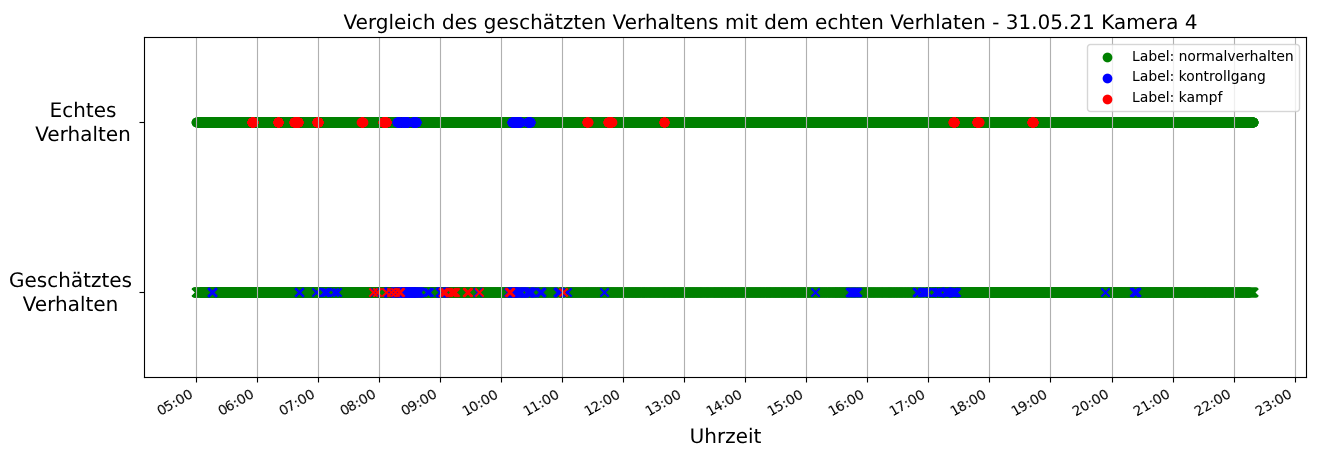
\includegraphics[width=\textwidth]{img/Plots/Simulation/Zeitstrahl Vergleich 31.05.21 cam 4.png}
         \caption{31.05.21 Kamera 4}
     \end{subfigure}
     \hfill
     \begin{subfigure}[b]{0.9\textwidth}
         \centering
         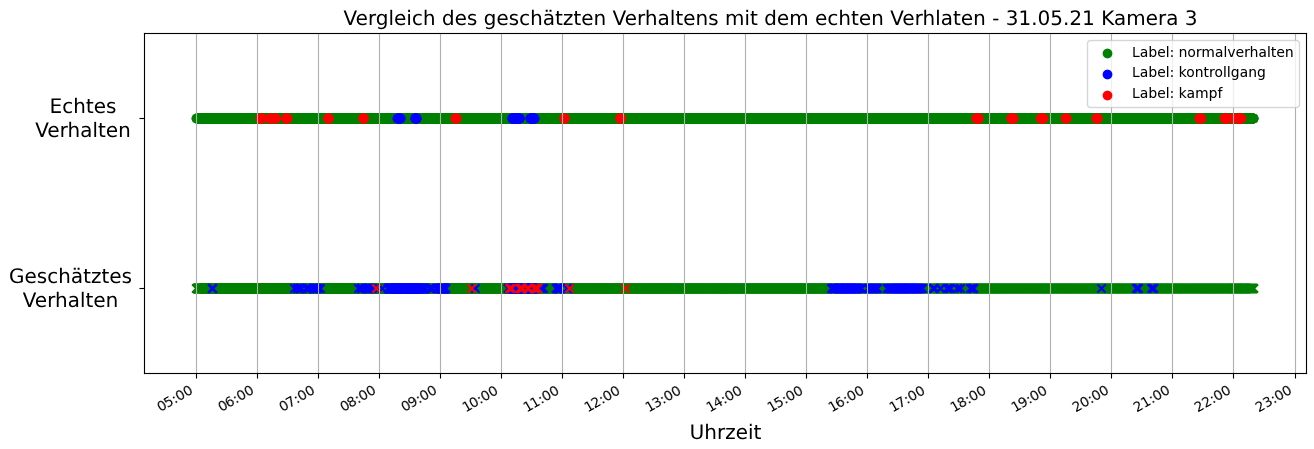
\includegraphics[width=\textwidth]{img/Plots/Simulation/Zeitstrahl Vergleich 31.05.21 cam 3.png}
         \caption{31.05.21 Kamera 3}
     \end{subfigure}
     \caption{Zeitstrahlen des Vergleichs von Klassifikation und Referenz.}
     \label{fig:zeitStrahlen}
\end{sidewaysfigure}


In der Abbildung \ref{fig:zeitStrahlen} ist gut zu sehen, dass die Kontrollgänge korrekt erkannt werden, jedoch auch, dass gerade nachmittags eine Überempfindlichkeit auftritt. Normalverhalten wird als Kontrollgang erkannt. Ebenfalls fällt auf, dass das Normalverhalten das Stallgeschehen dominiert. Das war zu erwarten, jedoch kann dies die Auswertung verzerren. Ein Modell, welches immer Normalverhalten schätzt, liegt dadurch trotzdem die meiste Zeit richtig. Die Bewertung ist somit zugunsten der Erkennung von Normalverhalten verzerrt. \par

Da die Trainingsdatenenge nicht besonders hoch ist, kann es sein, dass die Kampfereignisse nicht repräsentativ genug sind, um eine Generalisierung zu ermöglichen. Da die Evaluierung des Modells kein Overfitting aufweist (\autoref{sec:ErgebModSelEval}) ist es möglich, dass ein ungewollter Bias im Datensatz vorhanden ist, welcher durch geringe Varianz entsteht. Auch kann die geringe Datenmenge dafür sorgen, dass das Evaluationsergebnis nicht repräsentativ ist. Die Menge im Testdatensatz kann eine zu geringe Varianz haben, um die Generalisierung des Modells aussagekräftig zu prüfen. Die deutlichen Schwankungen in der Accuracy beim Validieren, können darauf hindeuten.\par

Zusätzlich ist es möglich, dass die Features nicht gut darin sind, die eindeutigen Charakteristiken der Kämpfe einzufangen. Viele der Features zielen auf die Gruppendynamik ab. Für die Identifikation der lokalen Dynamiken sind eventuell spezieller Features notwendig. Ein weiteres Hindernis für die Erkennung von lokalen Dynamiken kann die Komprimierung der Zeitreihen sein. Da bei Kämpfen ein Großteil der Tiere sich eher normal verhält, kann es sein, dass die Kampf-Merkmale nicht deutlich genug zum Vorschein kommen. \par


\subsection{Fazit der Simulationsauswertung}
Das Modul ist auf Basis der Anforderungen als Echtzeitfähig einzustufen. Zwischen Beginn eines Ereignisses und der Erkennung liegen zwischen 33,33 Sekunden und 40,46 Sekunden. Die Abtastrate beträgt im Mittel 4,14 Sekunden. Das Modul läuft stabil und kann konstant den Datenstrom eines Kamerabereichs von einem ganzen Tag verarbeiten. \par

Die Verhaltensklassifizierung ist unzuverlässig. Kämpfe werden nicht erkannt. Hauptgrund sind vermutlich die geringe Datenmenge, unzureichende Features und die Komprimierung der Zeitreihen. Kontrollgänge werden zuverlässig erkannt, wenn auch eine Überempfindlichkeit vorhanden ist. Das bestätigt jedoch, dass eine Verhaltenserkennung möglich ist. Die Auswertung der Simulationsergebnisse besitzt eine Verzerrung zugunsten des Normalverhaltens. 